% Created 2020-09-30 Wed 15:22
% Intended LaTeX compiler: pdflatex
\documentclass[10pt,t]{beamer}
\usepackage[utf8]{inputenc}
\usepackage{graphicx}
\usepackage{grffile}
\usepackage{longtable}
\usepackage{wrapfig}
\usepackage{rotating}
\usepackage{textcomp}
\usepackage{amssymb}
\usepackage{capt-of}
\usepackage{hyperref}
\usetheme{default}
%
\usepackage[font=small,labelfont=bf]{caption} % Required for specifying captions
%
\author{C. L. Hepplewhite}
\date{\today}
\title{\large Radiative Transfer Algorithm Updates}
\subtitle{\footnotesize{AIRS Virtual Science Team Meeting}}
\date{\vspace{0.1in}\footnotesize{October 2020 \vfill}}
\author{C. L. Hepplewhite\inst{1,2}, L. Larrabee Strow\inst{1,2}, and S. deSouza Machado\inst{1,2}  and thank to Bill Irion (JPL)}
\institute[UMBC]{\inst{1} UMBC Physics Dept. \and \inst{2}UMBC JCET}
\input beamer_setup
\metroset{titleformat title=allcaps}
\setbeamertemplate{frame footer}{UMBC Atmospheric Spectroscopy Lab}
\begin{document}

\maketitle

% -----------------------------------------------------
\begin{frame}{Introduction}
  \begin{itemize}
  \item Current and upcoming set of SARTA builds 
  \item Possible future improvements 
  \item Minor fitting improvements
  \item RTA/HITRAN intercomparisons over time and tuning issues
  \end{itemize}

\end{frame}
% ----------------------------------------------------
\begin{frame}{Current Spectroscopy}
  \begin{itemize}
  \item HITRAN 2016
  \item CO2, CH4 line mixing from LBLRTM12.8
  \item MT CKD3.2
  \item CO2 CIA from WV and N2 by Hartmann (4.3 um)
    \begin{itemize}
    \item Will affect T(z) retrievals using shortwave, needs testing
    \end{itemize}
  \item Single parameter surface emissivity.
  \item Used in IASI, AIRS L1c, and CHIRP RTAs.
  \end{itemize}
\end{frame}
% -------------------------------------------------
\begin{frame}{Current SARTAs at ASL}

  \begin{itemize}
  \item The following SARTAs are in use at ASL:
    Dates are release dates.
    \begin{itemize}
    \item AIRS L1B (2008):  Used in AIRS V6, V7 Level 2
    \item AIRS L1C (2019):  Possible use by Bill Irion, CLIMCAPS
    \item CrIS NSR v2012, \& v2016  
    \item CrIS FSR v2016
    \item IASI v2008 and v2016
    \item CHIRP v2020
    \end{itemize}
  \end{itemize}

\end{frame}
% ---------------------------------------------------
\begin{frame}{Future Improvements/Activities}

  \begin{itemize}
  \item HITRAN 2020, should be out this year.
  \item Line Mixing package from the HITRAN (Iouli Gordon, Harvard-Smithsonia).
  \item Currently use kCARTA at 0.0025 cm-1 steps, can move to 0.0005 cm-1 step in 15 \um region
  \item Interpolation improvements in kCARTA
  \item Nalli surface emissivity parameterization?  Under study.
  \item Improved non-LTE, the extreme solar angles.  Not yet started.
  \item RTA tuning in collabortion with Chris Barnet and Bill Irion (more later in talk)
  \item Hope to perform major re-validation on new RTAs using HITRAN 2020, probably last time...
  \end{itemize}
\end{frame}

% ------------------------------------------------
\begin{frame}[shrink=5]{Validation: Fitting Accuracy}

%Here concentrate just on fitting accuracy.  Future work on independent validation using re-analysis, sondes, etc.

\begin{itemize}
    \item Fast coefficients are checked by comparing top-of-atmosphere (TOA) radiances predicted by SARTA and kCARTA.
   \end{itemize}
    \begin{center}
    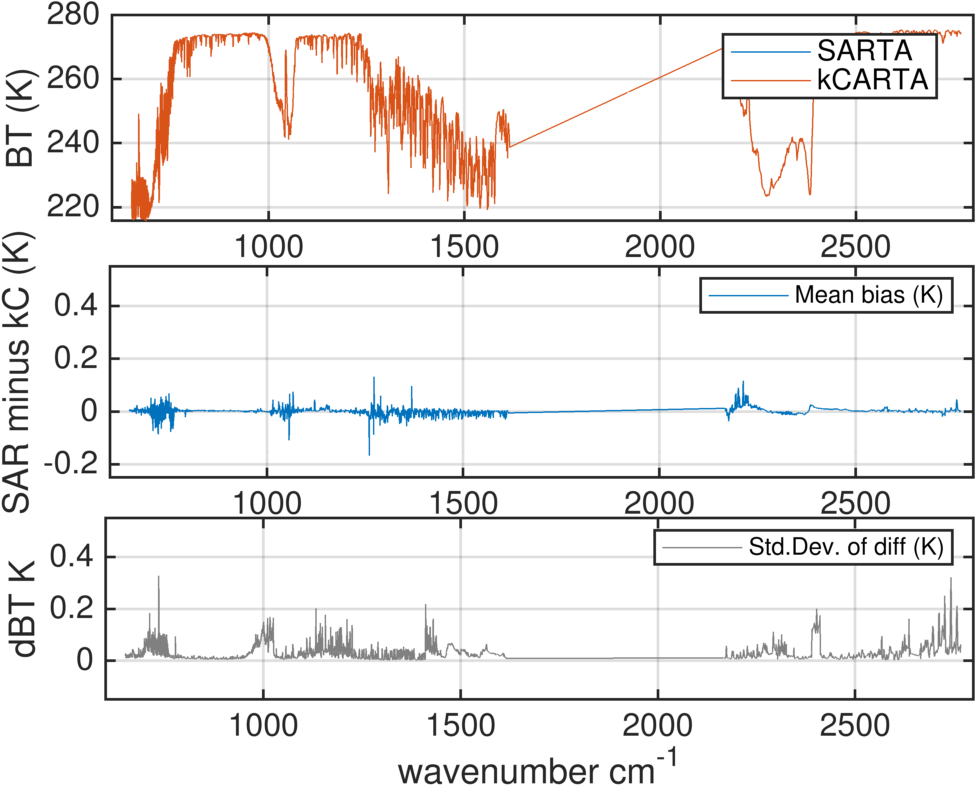
\includegraphics[width=0.6\linewidth]{./Figs/kc_sar_airs_l1c_mean_bias_stdv_sea_6angs_aslp.png}
    \captionof{figure}{AIRS bias relative to kCARTA.}
  \end{center}
  
\end{frame}
% -----------------------------------------------
%\begin{frame}[shrink=10]{Improved bias \& std.dev relative to kCARTA}
\begin{frame}{Improved bias \& std.dev relative to kCARTA}

  \begin{itemize}
  \item SARTA parameterization based on ratios of convolved kCARTA monochromatic layer-so-space transmittances.
  \item AIRS SRF (convolution) produced well-behaved layer-averaged transmittances/optical depths.
  \item Residual since ringing from interferometers (IASI, CrIS, CHIRP) occasionally produce negative optical depths, which are ignore via a threshold that is slightly above zero.
  \item Last set of  IASI, CrIS, and CHIRP RTA builds exhibited ~0.2K biases errors in certain regions due to this threshold being too high.
  \item These problems are now fixed, for the most recent set of SARTA builds and for CHIRP.
  \end{itemize}

\end{frame}

% -----------------------------------------------
\begin{frame}{Example of optimization: CHIRP 640 cm-1}
\vspace{-0.1}
  \begin{center}
    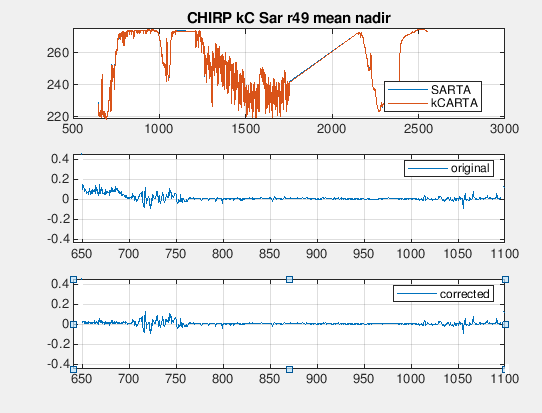
\includegraphics[width=0.75\linewidth]{./Figs/chirp_optimize1_edit.png}
    \captionof{figure}{CHIRP SARTA bias compared to kCARTA, with and without improved regression.}
  \end{center}


\end{frame}
% -----------------------------------------------
\begin{frame}[shrink=5]{Example of optimization: IASI $2300 cm^{-1}$}

\vspace{-0.5cm}
  \begin{center}
    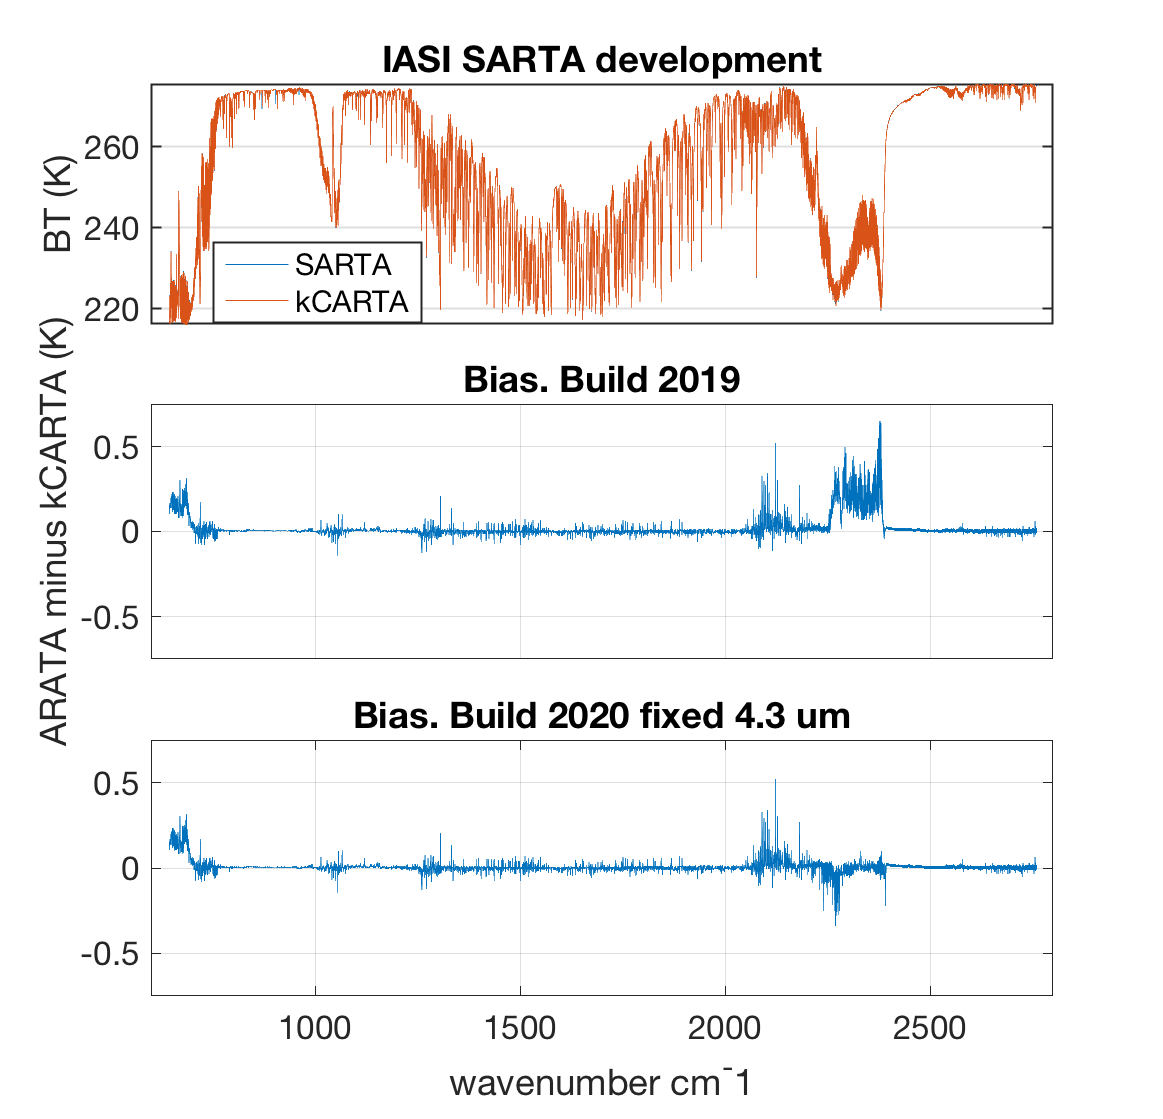
\includegraphics[width=0.6\linewidth]{./Figs/iasi_sarta_kcarta_mean_bias_4p3um_fx.png}
    \captionof{figure}{IASI SARTA bias compared to kCARTA, with and without improved regression at 2300 cm$^{-1}$. Problem at 650 cm$^{-1}$ is now fixed as well.}
  \end{center}

\end{frame}
% -----------------------------------------------
\begin{frame}{Tuning}

  \begin{block}{}
  Retrieval and NWP assimilation require Obs - Fit bias removal, via ``tuning'' Bias can occur because of:  
  \end{block}
    
  \begin{itemize}
  \item AIRS radiometric calibration.
  \item AIRS spectral calibration and instrument line shape.
  \item AIRS fast model parameterization.
  \item Spectroscopy (including continuum and lineshape)
  \item Cloud contamination in fields of view selected as clear
  \item Validation data, including time/space mismatches and uncertainties in minor gas abundances.
  \end{itemize}

Two approaches: (a) Tune the spectroscopy (optical depths), (b) Tune the (Obs - Calc) B(T)'s.
  
\end{frame}
% -----------------------------------------------
% \begin{frame}{Tuning: 2}

%   \begin{block}{}
%     The objective of tuning is to reduce bias in the real world sufficiently to increase the yield in single footprint geophysical retrievals.
%   \end{block}

%   \begin{itemize}
%   \item Large data sets are compared covering all global atmospheric and scene types.
%   \item Bias and std.dev characterisctics between coincident TOA measurements with forward model predictions are determined.
%   \item RTA transmittances are adjusted for specific channels where needed.
%   \item SARTA uses a supporting data file of tuning parameters.
%   \item Tuning of transmittances in the RTA are preferred over tuning BT of TOA predicts.

%   \end{itemize}

% \end{frame}
% % ----------------------------------------------
% \begin{frame}{Recent Tuning Studies}

%   \begin{block}{}
%   \end{block}

%   \begin{itemize}

%   \end{itemize}

% \end{frame}

%

\begin{frame}[label={sec:org472f9d3}]{Recent Tuning Studies (with Bill Irion)}

Immediate motivation: Help Bill Irion use AIRS L1c and associated AIRS L1c RTA

\begin{itemize}
\item 17 days of AIRS clear ocean scene radiances are compared to ECMWF simulations
\item Three RTA variants tested:
\begin{itemize}
\item L1c RTA  (``L1c'')
\item L1b RTA as tuned for V6 Level 2 retrievals, (``L1b tuned'')
\item L1b RTA without tuning  (``L1b'')
\end{itemize}
\item The L1c RTA uses HITRAN 2016 and new (improvements?) to the continuum and line mixing
\item The L1b RTA is circa 2008
\item Conclusions here assume ECMWF is "truth".  Better than 5\% --> 0.3K?  Is ECMWF the truth?
\end{itemize}
\end{frame}

\begin{frame}[label={sec:orgf207f3e}]{Longwave Biases}
\begin{center}
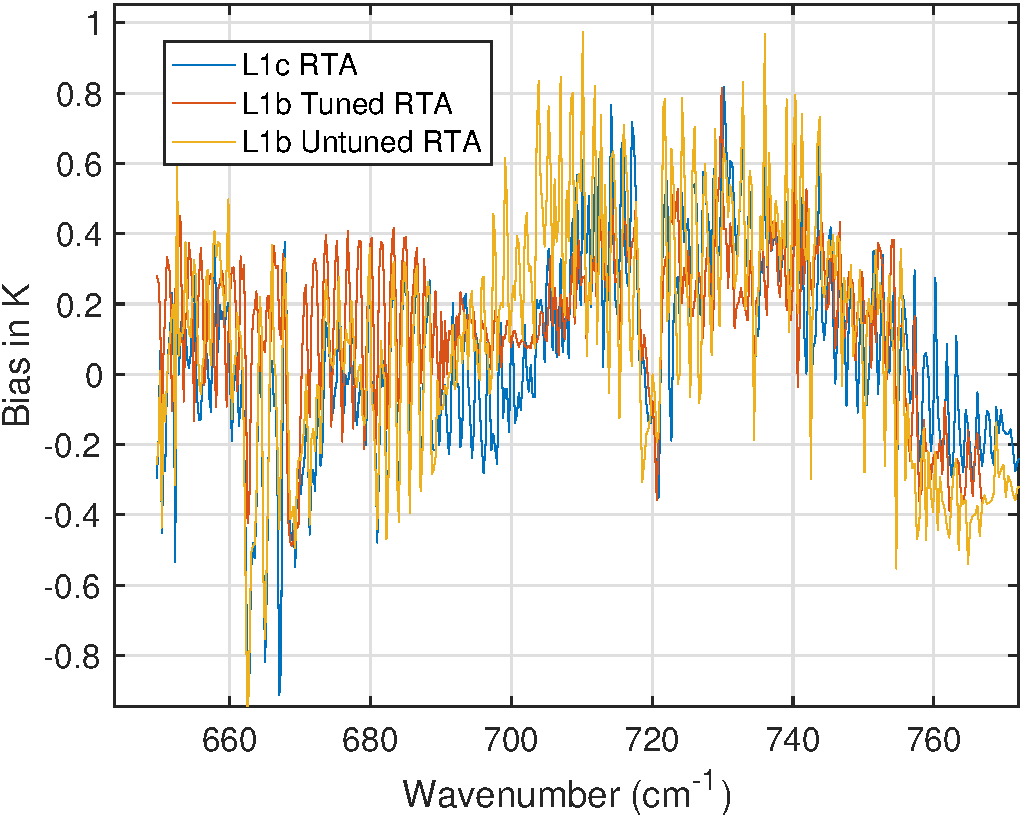
\includegraphics[width=0.75\linewidth]{./Talk2/bias_3rta_lw.pdf}
\end{center}
\end{frame}

\begin{frame}[label={sec:org87db84f},noframenumbering]{Longwave Biases}
\begin{center}
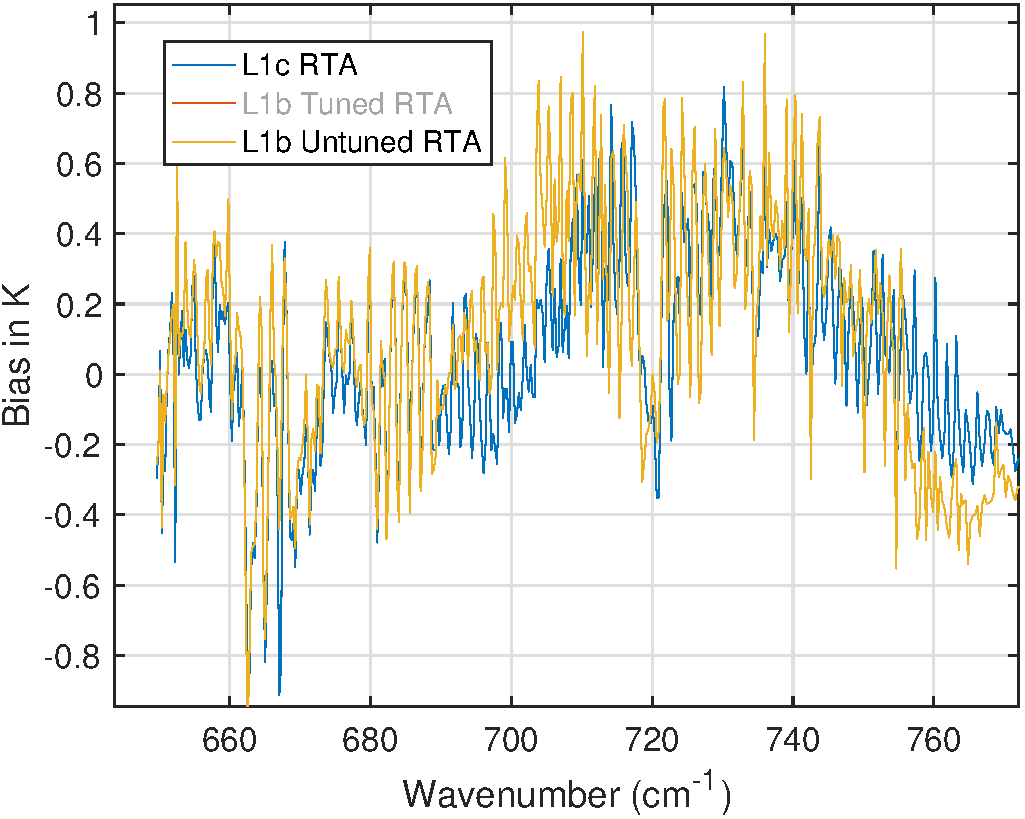
\includegraphics[width=0.75\linewidth]{./Talk2/bias_3rta_lw_noL1btuning.pdf}
\end{center}
%L1c RTA appears a bit better.  (Note fill channels included!)
\end{frame}

\begin{frame}[label={sec:org2af980b},noframenumbering]{Longwave Biases}
\begin{center}
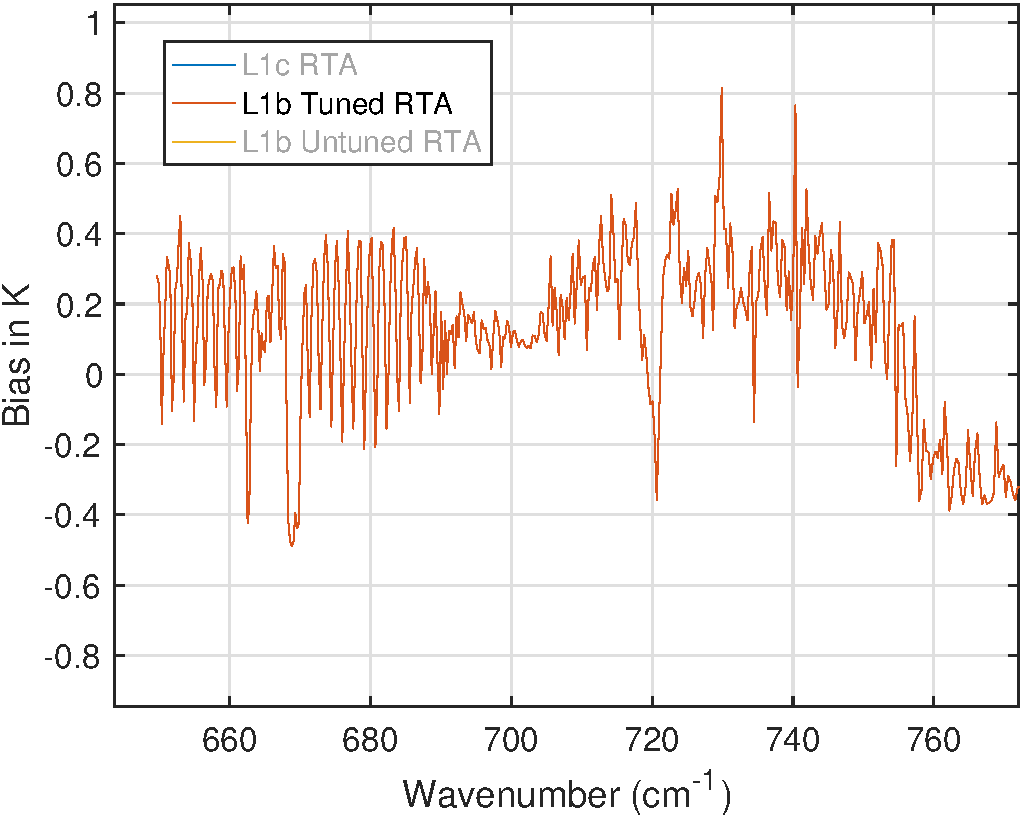
\includegraphics[width=0.75\linewidth]{./Talk2/bias_3rta_lw_justL1btuning.pdf}
\end{center}
\end{frame}


\begin{frame}[label={sec:org68cebb3}]{Midwave Biases}
\begin{center}
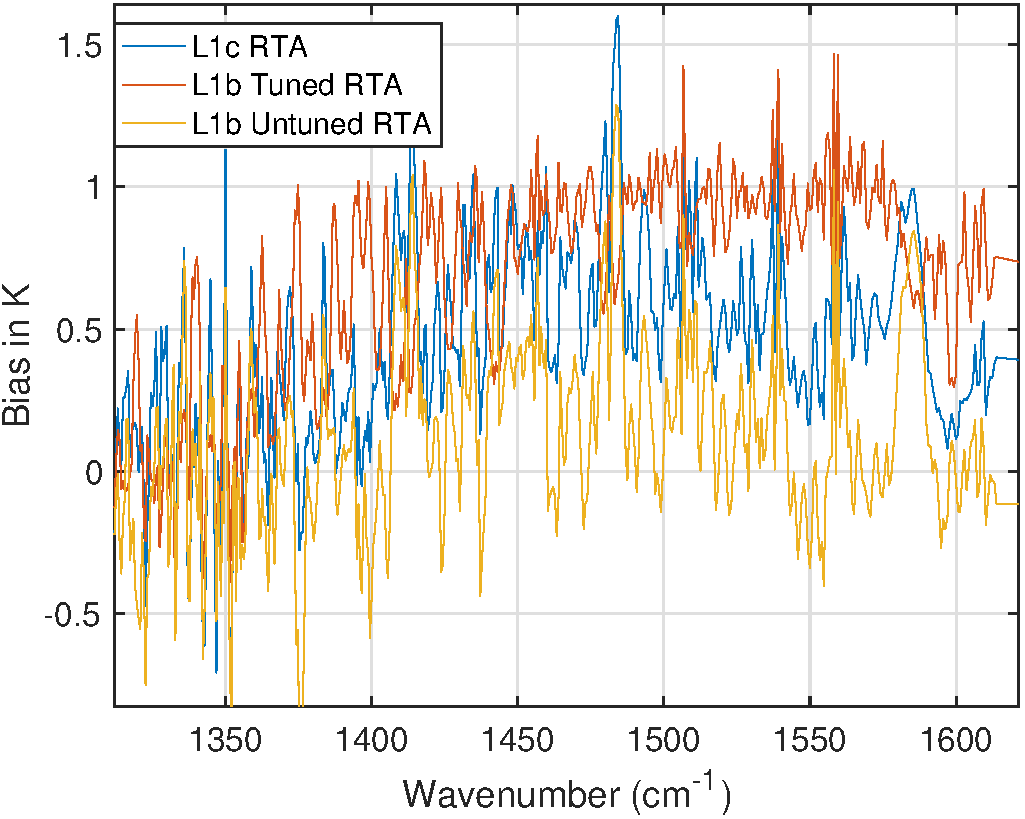
\includegraphics[width=0.75\linewidth]{./Talk2/bias_3rta_mw.pdf}
\end{center}
\end{frame}

\begin{frame}[label={sec:org5d2824b}]{Midwave Biases}
\addtocounter{framenumber}{-1}
  \begin{center}
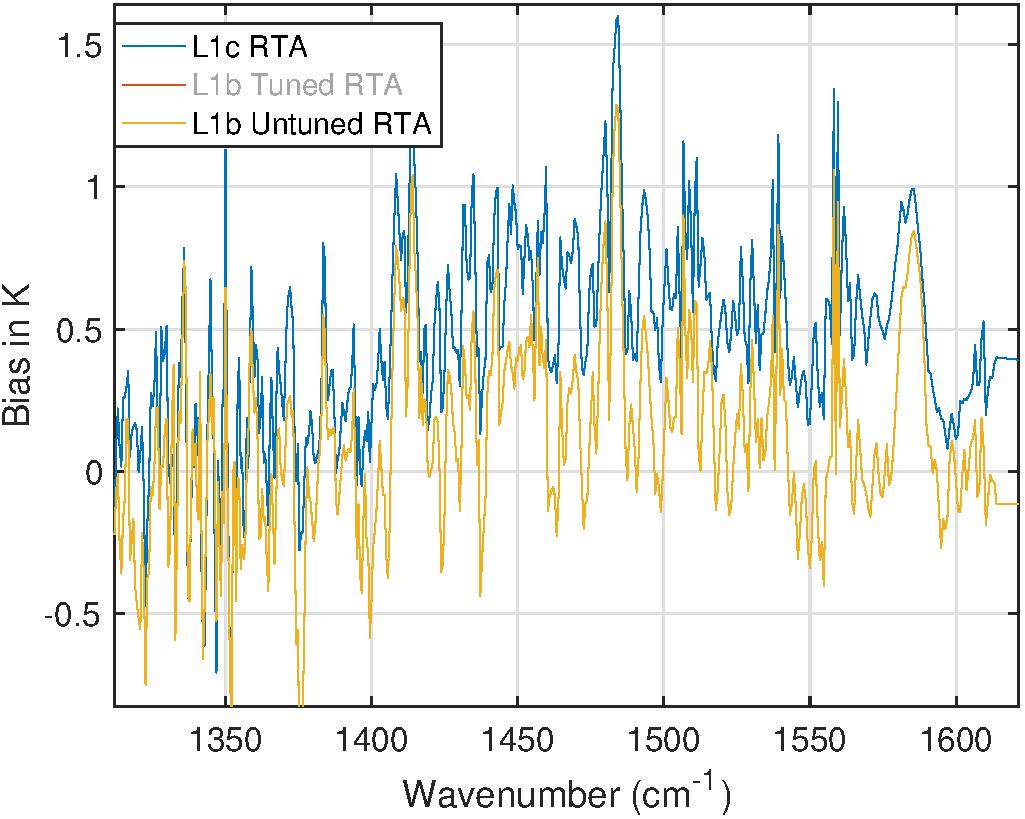
\includegraphics[width=0.75\linewidth]{./Talk2/bias_3rta_mw_noL1btuning.pdf}
\end{center}
\end{frame}

\begin{frame}[label={sec:org22ce356}]{Midwave Biases}
\addtocounter{framenumber}{-1}
  \begin{center}
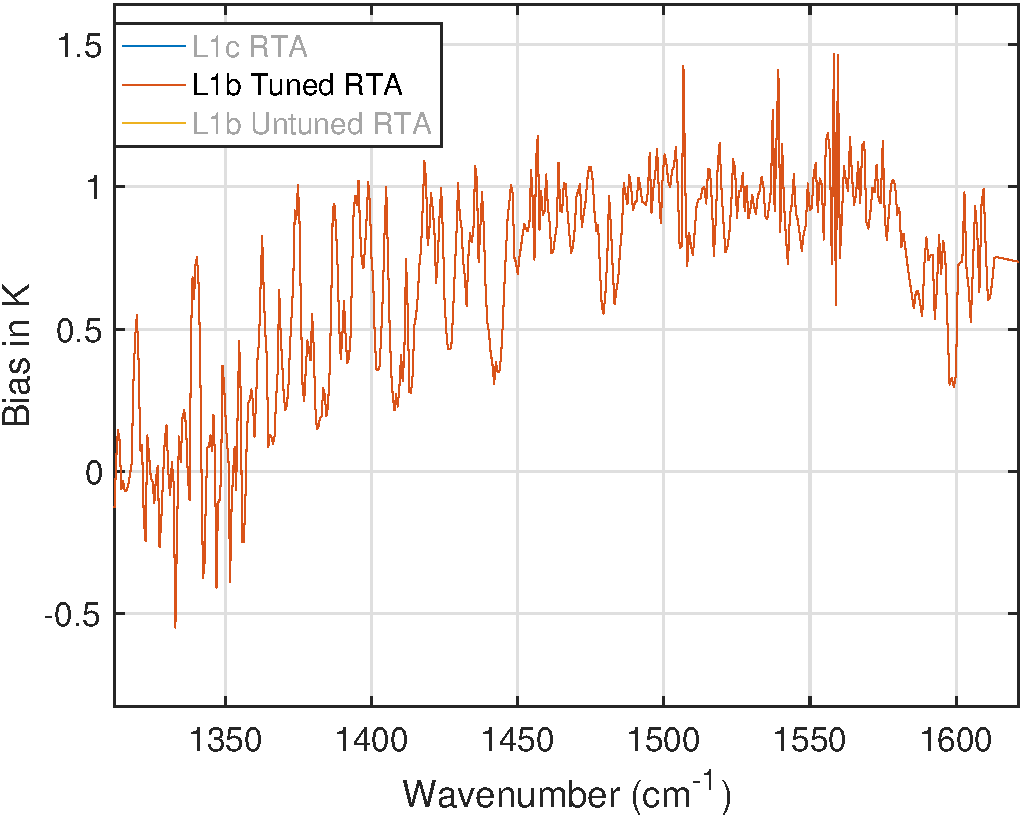
\includegraphics[width=0.75\linewidth]{./Talk2/bias_3rta_mw_justL1btuning.pdf}
\end{center}
\end{frame}

\begin{frame}[label={sec:org047c8ba}]{650-700 \wn Biases vs BTobs}
\begin{center}
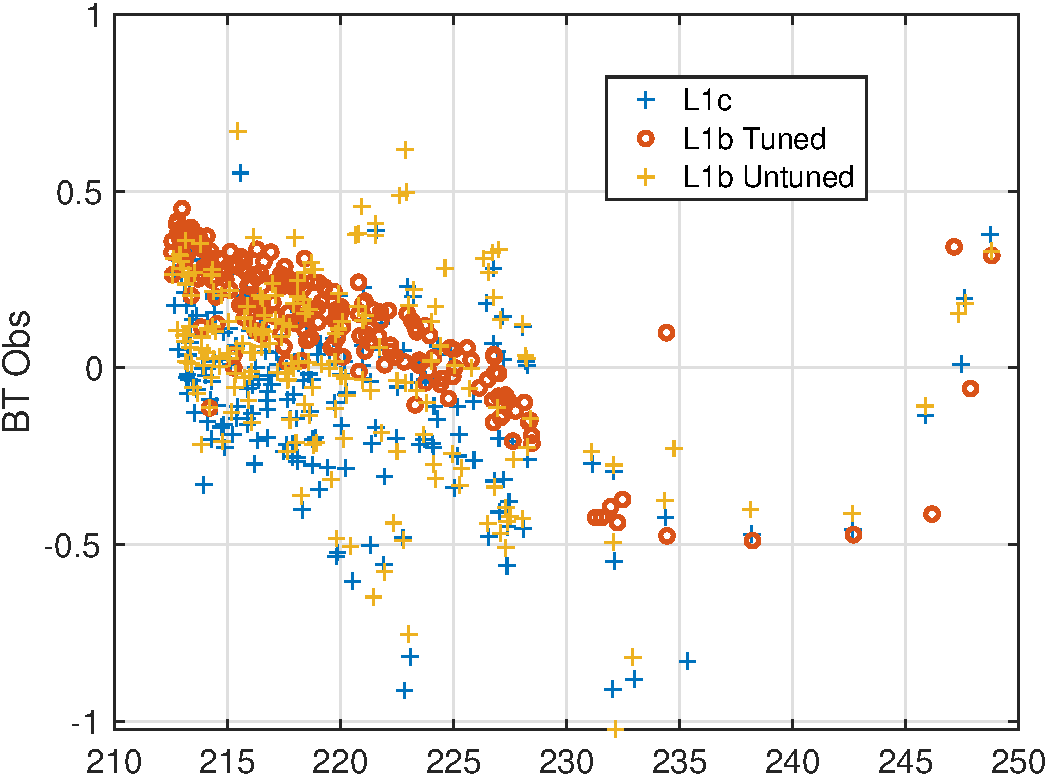
\includegraphics[width=0.75\linewidth]{./Talk2/bias_vs_btobs_650-700.pdf}
\end{center}
\end{frame}

\begin{frame}[label={sec:org6447e1f}]{1320-1614 \wn Biases vs BTobs}
Similarly for water band, L1b tuned has a clear bias dependence on BTobs
\begin{center}
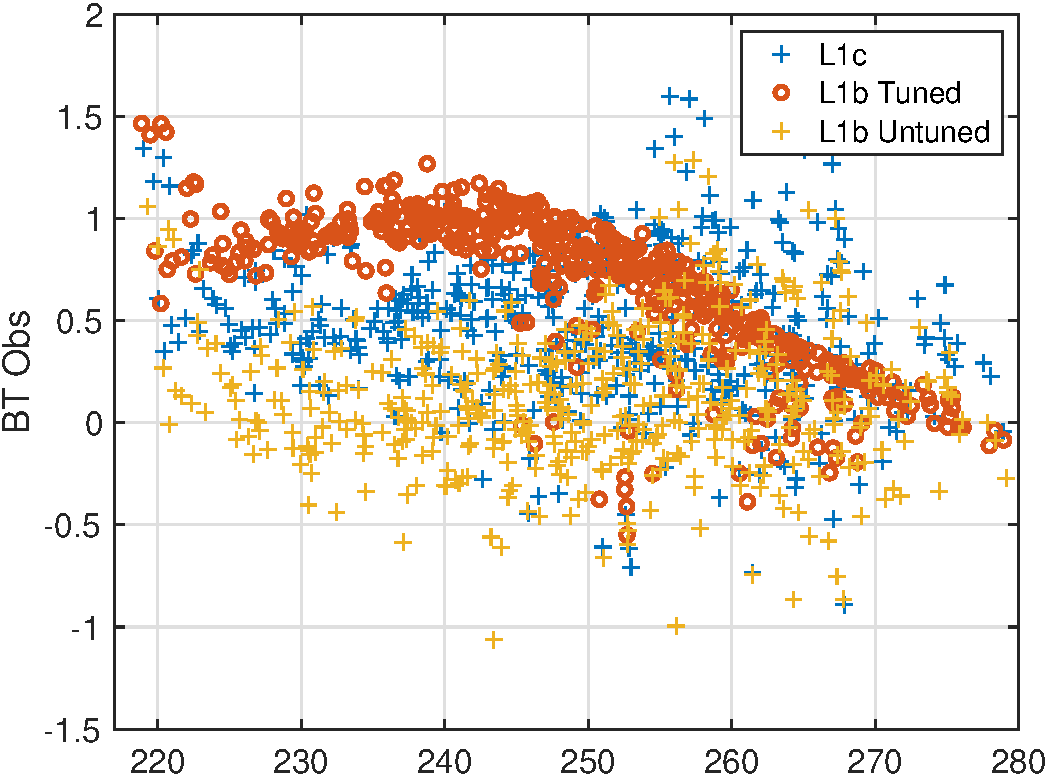
\includegraphics[width=0.75\linewidth]{./Talk2/bias_vs_btobs_1320-1614.pdf}
\end{center}
\end{frame}

\begin{frame}[label={sec:org9697316}]{Longwave Bias Std. Devs. (with Latitude)}
\begin{center}
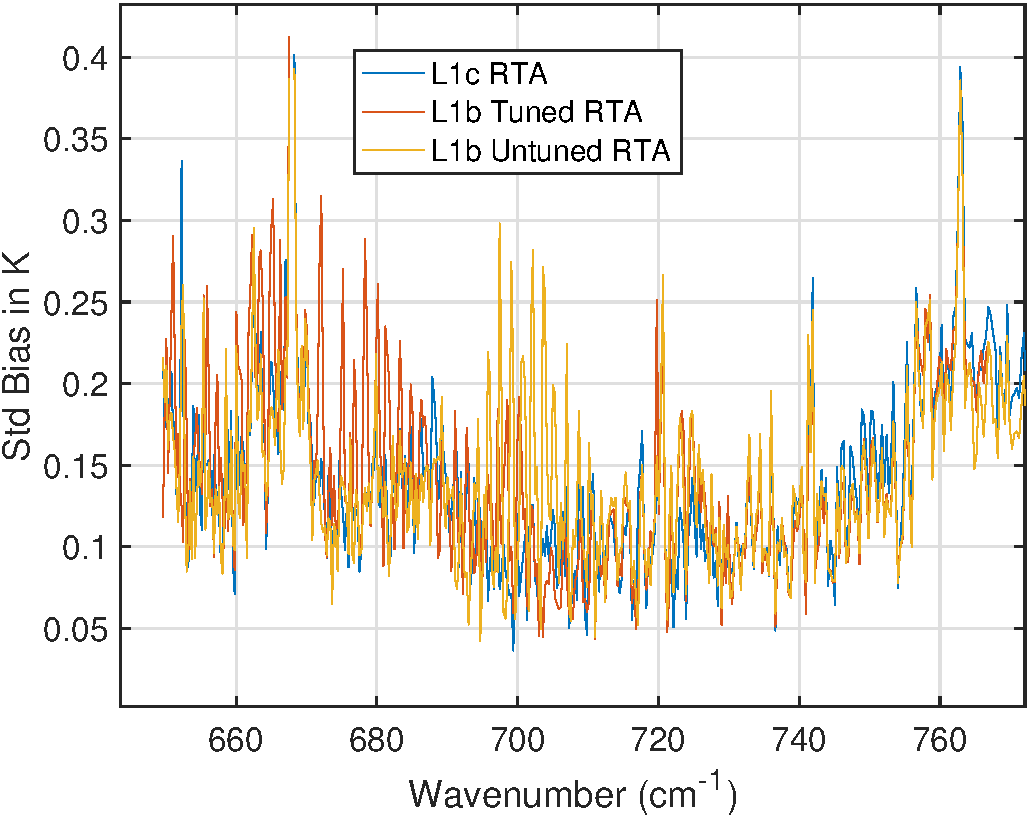
\includegraphics[width=0.75\linewidth]{./Talk2/std_3rta_lw.pdf}
\end{center}
\end{frame}

\begin{frame}[label={sec:org0f46d77}]{Longwave Bias Std. Devs. (with Latitude)}
\addtocounter{framenumber}{-1}
  \begin{center}
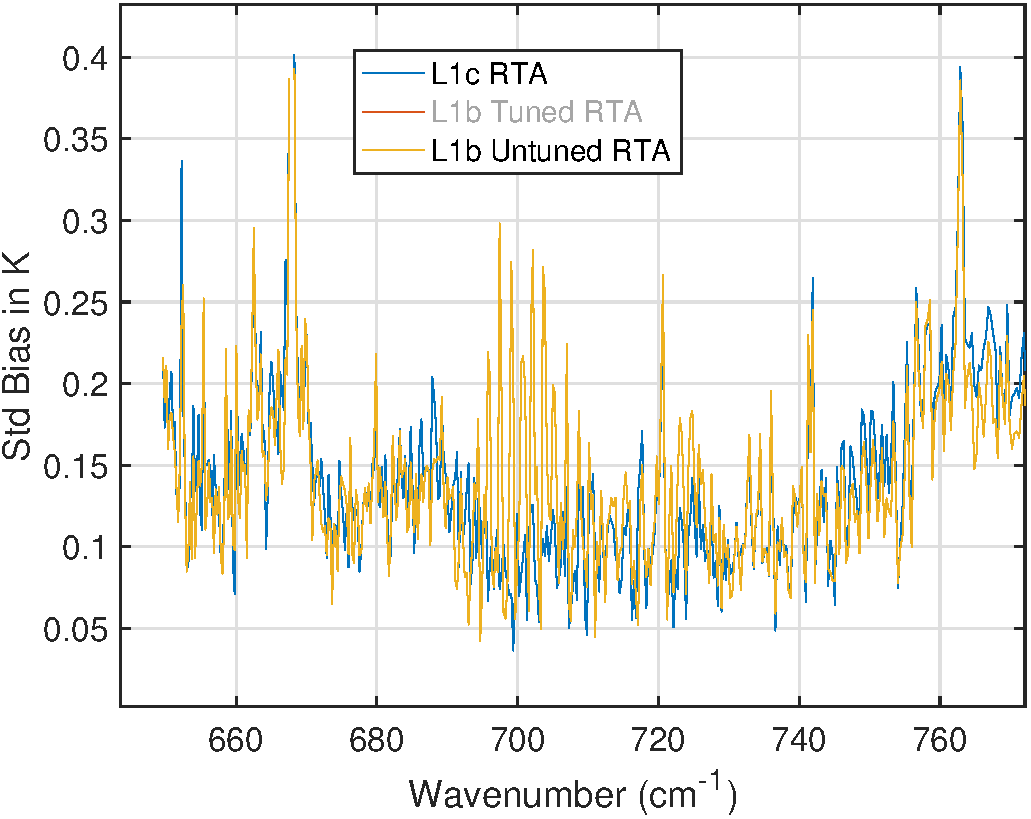
\includegraphics[width=0.75\linewidth]{./Talk2/std_3rta_lw_noL1btuning.pdf}
\end{center}
\end{frame}

\begin{frame}[label={sec:orga29dad3}]{Longwave Bias Std. Devs. (with Latitude)}
\addtocounter{framenumber}{-1}
  \begin{center}
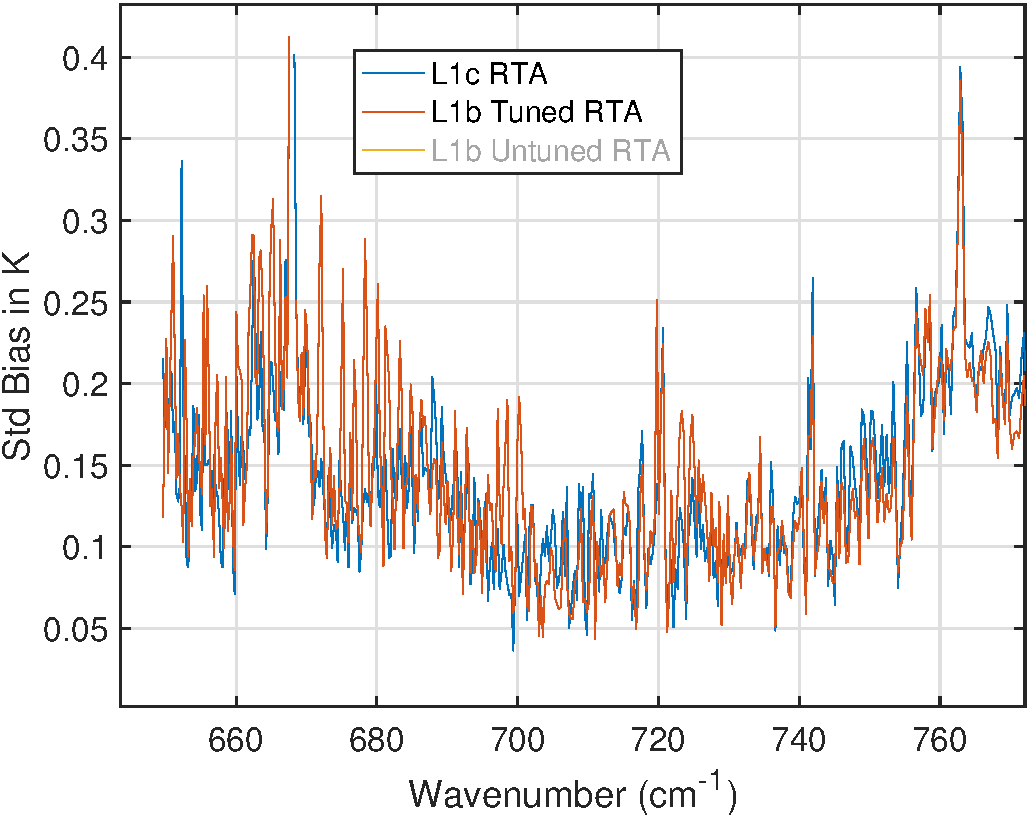
\includegraphics[width=0.75\linewidth]{./Talk2/std_3rta_lw_nol1b_untuned.pdf}
\end{center}
\end{frame}

\begin{frame}[label={sec:orgfcad398}]{Midwave Bias Stds  (with Latitude)}
\begin{center}
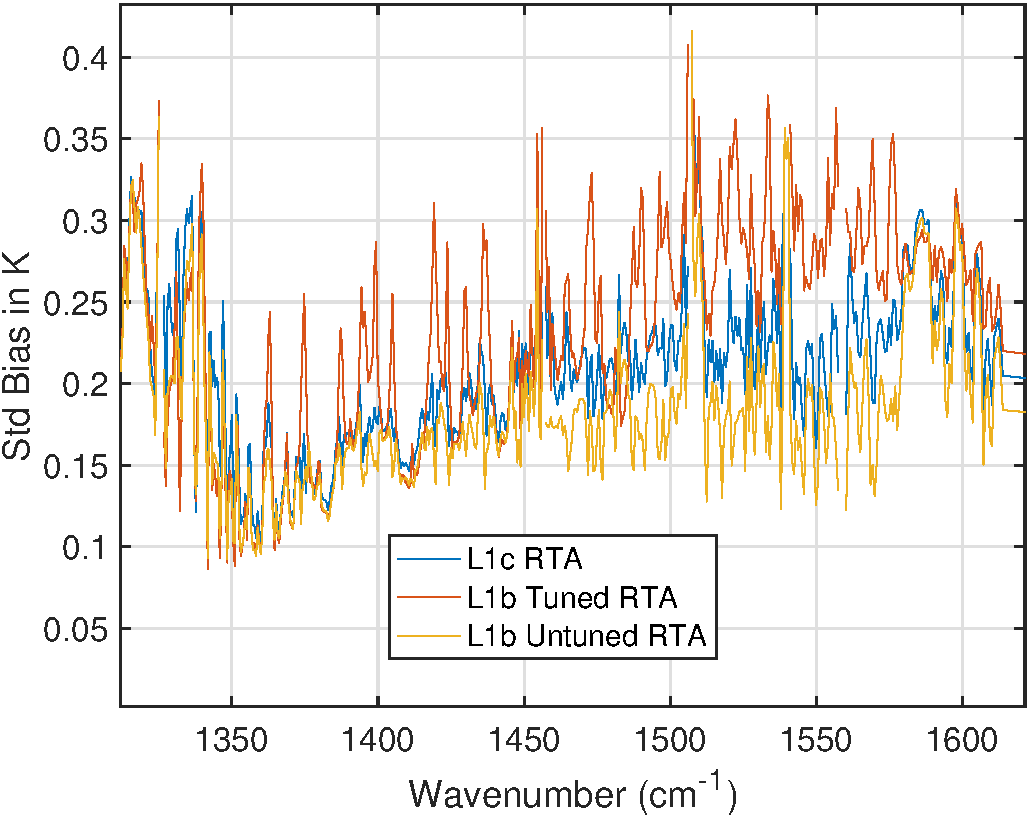
\includegraphics[width=0.75\linewidth]{./Talk2/std_3rta_mw.pdf}
\end{center}
\end{frame}

\begin{frame}[label={sec:org6edc0cf}]{Midwave Bias Stds  (with Latitude)}
\addtocounter{framenumber}{-1}
  \begin{center}
  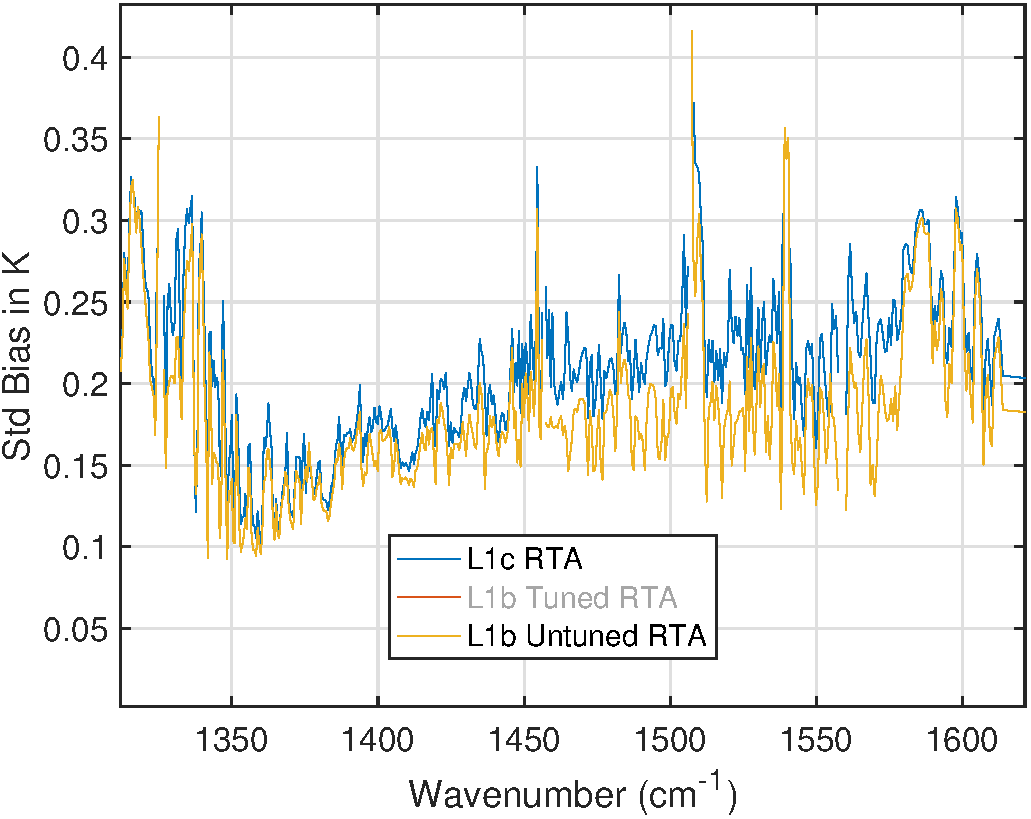
\includegraphics[width=0.75\linewidth]{./Talk2/std_3rta_mw_noL1btuning.pdf}
\end{center}
\end{frame}

\begin{frame}[label={sec:org916b712}]{Midwave Bias Stds}
\addtocounter{framenumber}{-1}
  \begin{center}
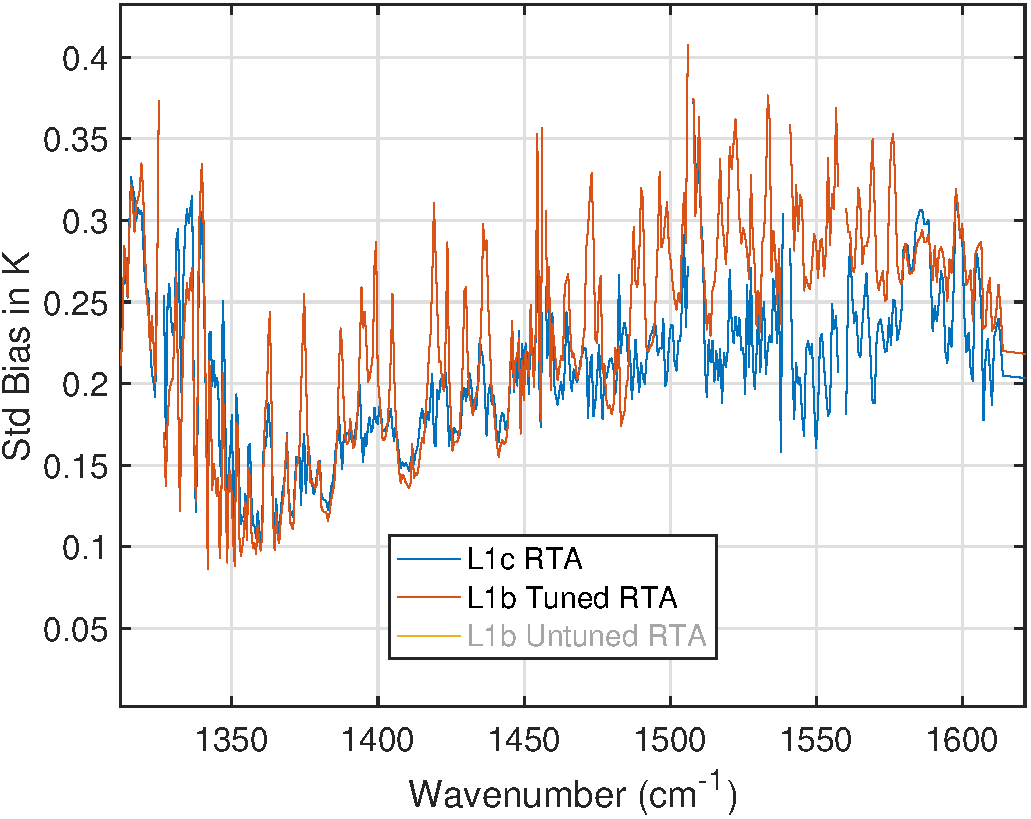
\includegraphics[width=0.75\linewidth]{./Talk2/std_3rta_mw_nol1b untuned.pdf}
\end{center}
\end{frame}

\begin{frame}[label={sec:org8aa77db}]{1320-1614 \wn Bias Stds versus BTobs}
Scene dependence of STD, clear increase for cold scenes for L1b Tuned RTA
\begin{center}
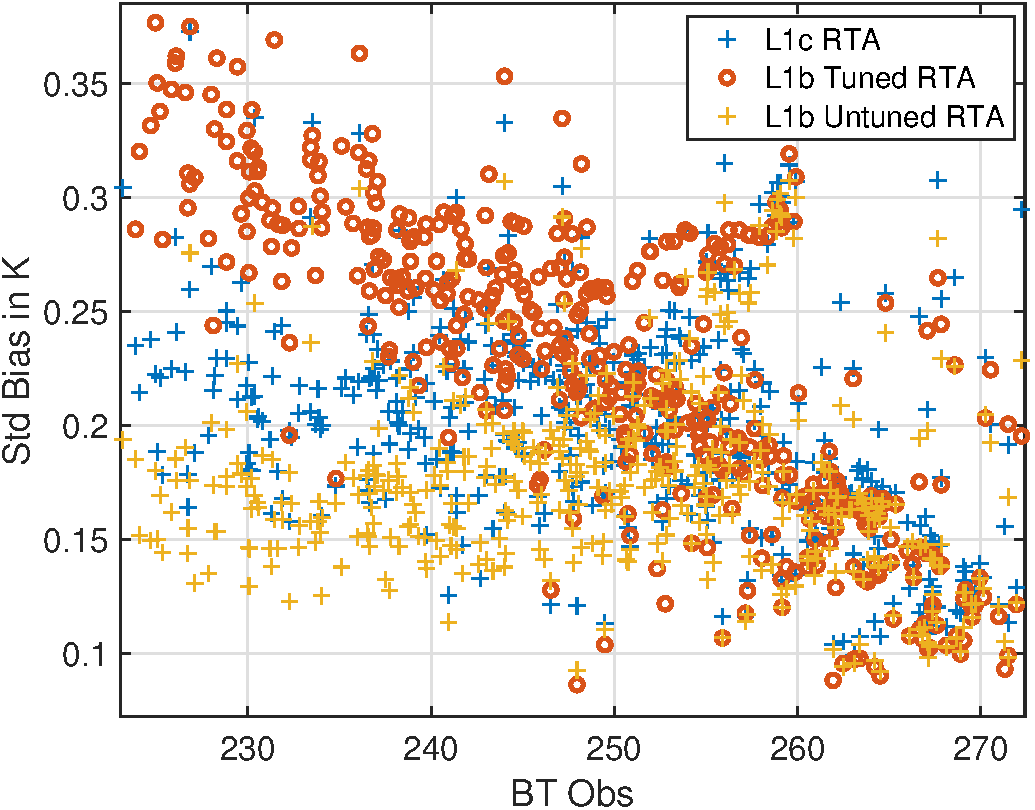
\includegraphics[width=0.75\linewidth]{./Talk2/std_vs_btobs_1320-1614.pdf}
\end{center}
\end{frame}

\begin{frame}[label={sec:orgcfca8da}]{Final Effect: L1btuning RTA + Level 2 BT Tuning}
\begin{itemize}
\item V6 Level 2 retrieval uses tuned RTA \alert{BUT}
\item It also does BT tuning.
\item Except in longwave, they cancel each other out!  NOT GOOD.
\end{itemize}
\begin{center}
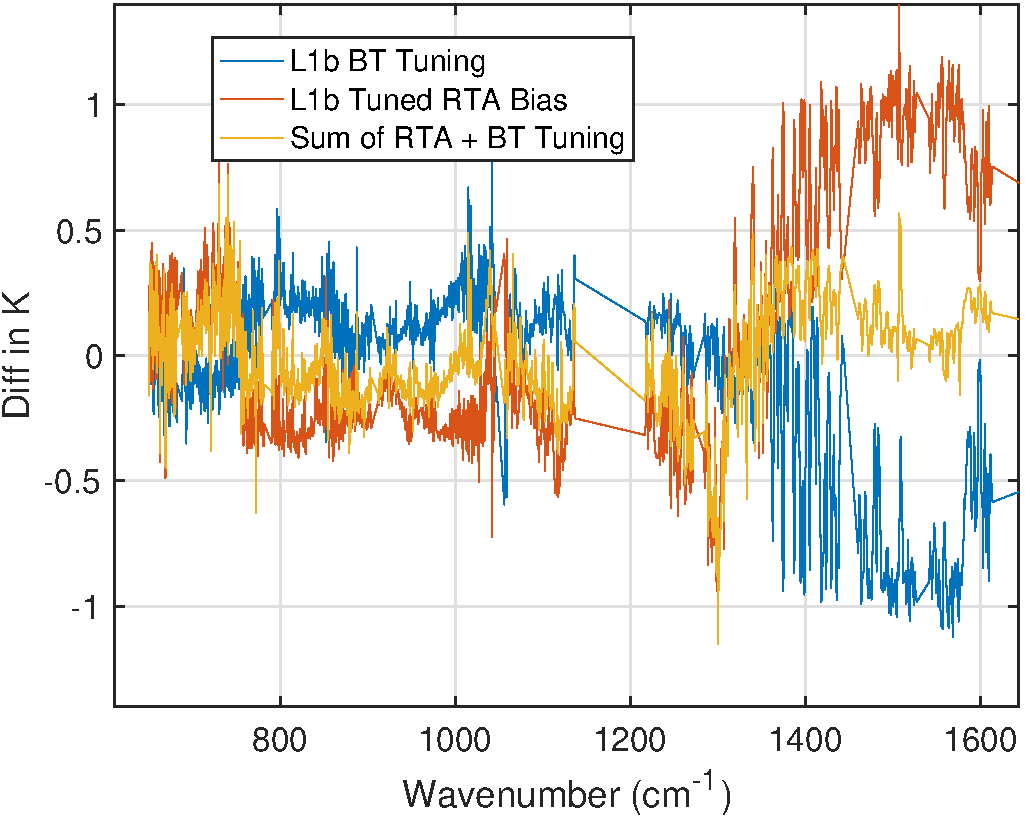
\includegraphics[width=0.65\linewidth]{./Talk2/l1b_bttuning_l1b_tunedbias_added.pdf}
\end{center}
\end{frame}

\begin{frame}{Tuning Summary}
\begin{itemize}
\item Longwave (CO$_2$)
  \begin{itemize}
  \item Biases and Stds: L1c better in general than L1b and L1b-tuned
  \end{itemize}
\item Midwave (water)
  \begin{itemize}
  \item Biases:  L1b better in general than L1c, L1b tuned bias quite bad
  \item Stds: L1b slightly lower than L1c, L1b tuned quite bad
  \item B(T) tuning:  L1b tuned bias errors ``compensated'' by static B(T) tuning!  Not good.
  \end{itemize}
\end{itemize}

Do we just assume ECMWF is correct?

How much effort should be put into radiosonde validation?

If Level 2 efforts aimed at reproducing ECMWF, then radiosonde validation efforts not worth the work.
\end{frame}





% ----------------------------------------------
% \begin{frame}{Conclusions}

%   \begin{block}{}
%   \end{block}

%   \begin{itemize}

%   \item CHIRP SARTA now available although further validation at UMBC in progress.
%   \item New version of all RTAs planned using the new HITRAN 2020, although this assumes improvements to the relevant line parameters and line shape for AIRS/CrIS/CHIRP.
%   \item Extensive validation push is planned for the future, in concert with tuning exercises for all RTAs.  Water vapor tuning needs to be understood.
%   \item New lineshape in the 2400 cm$^{-1}$ region needs further validation.
    
    
%   \end{itemize}

% \end{frame}
% % -----------------------------------------------


\end{document}


% -----------------------------------------------------
\begin{frame}{The SARTA}

  \begin{itemize}
  \item The Stand-alone radiative transfer algorithm (SARTA) is constructed using kCARTA
  \item Therefore SARTA has the same spectroscopy as kCARTA.
  \item SARTA was developed 18 years ago for the AIRS.
  \item It uses sets of coefficients that parameterize atmospheric transmittances derived using a set of training profiles.
  \item Is written in Fortran
  \item Permits very fast computation of radiances for predefined spectral response functions.
    \item Has a version for clear sky radiance calculations and for cloudy radiances.
    
\end{itemize}

\end{frame}
% ----------------------------------------------------
\begin{frame}{Who uses SARTA}

  \begin{itemize}
  \item SARTA is used to compute clear and all-sky radiances for any and all FoVs from AIRS, CrIS and IASI missions.
  \item Is fast enough to make whole-mission modelling easily manageable. Faster than kCARTA *way* faster than LBL.
  \item Currently used in ASL for the RTP production for analysis of sensor performance and global studies and geophysical retireval.
  \item Is used in the AIRS geophysical product retrieval.
    \item Is used in NUCAPS.

  \end{itemize}
\end{frame}

%%% Local Variables:
%%% mode: latex
%%% TeX-master: t
%%% End:
